% Options for packages loaded elsewhere
\PassOptionsToPackage{unicode}{hyperref}
\PassOptionsToPackage{hyphens}{url}
\PassOptionsToPackage{dvipsnames,svgnames,x11names}{xcolor}
%
\documentclass[
  letterpaper,
  DIV=11,
  numbers=noendperiod]{scrartcl}

\usepackage{amsmath,amssymb}
\usepackage{iftex}
\ifPDFTeX
  \usepackage[T1]{fontenc}
  \usepackage[utf8]{inputenc}
  \usepackage{textcomp} % provide euro and other symbols
\else % if luatex or xetex
  \usepackage{unicode-math}
  \defaultfontfeatures{Scale=MatchLowercase}
  \defaultfontfeatures[\rmfamily]{Ligatures=TeX,Scale=1}
\fi
\usepackage{lmodern}
\ifPDFTeX\else  
    % xetex/luatex font selection
\fi
% Use upquote if available, for straight quotes in verbatim environments
\IfFileExists{upquote.sty}{\usepackage{upquote}}{}
\IfFileExists{microtype.sty}{% use microtype if available
  \usepackage[]{microtype}
  \UseMicrotypeSet[protrusion]{basicmath} % disable protrusion for tt fonts
}{}
\makeatletter
\@ifundefined{KOMAClassName}{% if non-KOMA class
  \IfFileExists{parskip.sty}{%
    \usepackage{parskip}
  }{% else
    \setlength{\parindent}{0pt}
    \setlength{\parskip}{6pt plus 2pt minus 1pt}}
}{% if KOMA class
  \KOMAoptions{parskip=half}}
\makeatother
\usepackage{xcolor}
\setlength{\emergencystretch}{3em} % prevent overfull lines
\setcounter{secnumdepth}{-\maxdimen} % remove section numbering
% Make \paragraph and \subparagraph free-standing
\makeatletter
\ifx\paragraph\undefined\else
  \let\oldparagraph\paragraph
  \renewcommand{\paragraph}{
    \@ifstar
      \xxxParagraphStar
      \xxxParagraphNoStar
  }
  \newcommand{\xxxParagraphStar}[1]{\oldparagraph*{#1}\mbox{}}
  \newcommand{\xxxParagraphNoStar}[1]{\oldparagraph{#1}\mbox{}}
\fi
\ifx\subparagraph\undefined\else
  \let\oldsubparagraph\subparagraph
  \renewcommand{\subparagraph}{
    \@ifstar
      \xxxSubParagraphStar
      \xxxSubParagraphNoStar
  }
  \newcommand{\xxxSubParagraphStar}[1]{\oldsubparagraph*{#1}\mbox{}}
  \newcommand{\xxxSubParagraphNoStar}[1]{\oldsubparagraph{#1}\mbox{}}
\fi
\makeatother


\providecommand{\tightlist}{%
  \setlength{\itemsep}{0pt}\setlength{\parskip}{0pt}}\usepackage{longtable,booktabs,array}
\usepackage{calc} % for calculating minipage widths
% Correct order of tables after \paragraph or \subparagraph
\usepackage{etoolbox}
\makeatletter
\patchcmd\longtable{\par}{\if@noskipsec\mbox{}\fi\par}{}{}
\makeatother
% Allow footnotes in longtable head/foot
\IfFileExists{footnotehyper.sty}{\usepackage{footnotehyper}}{\usepackage{footnote}}
\makesavenoteenv{longtable}
\usepackage{graphicx}
\makeatletter
\newsavebox\pandoc@box
\newcommand*\pandocbounded[1]{% scales image to fit in text height/width
  \sbox\pandoc@box{#1}%
  \Gscale@div\@tempa{\textheight}{\dimexpr\ht\pandoc@box+\dp\pandoc@box\relax}%
  \Gscale@div\@tempb{\linewidth}{\wd\pandoc@box}%
  \ifdim\@tempb\p@<\@tempa\p@\let\@tempa\@tempb\fi% select the smaller of both
  \ifdim\@tempa\p@<\p@\scalebox{\@tempa}{\usebox\pandoc@box}%
  \else\usebox{\pandoc@box}%
  \fi%
}
% Set default figure placement to htbp
\def\fps@figure{htbp}
\makeatother

\KOMAoption{captions}{tableheading}
\makeatletter
\@ifpackageloaded{caption}{}{\usepackage{caption}}
\AtBeginDocument{%
\ifdefined\contentsname
  \renewcommand*\contentsname{Table of contents}
\else
  \newcommand\contentsname{Table of contents}
\fi
\ifdefined\listfigurename
  \renewcommand*\listfigurename{List of Figures}
\else
  \newcommand\listfigurename{List of Figures}
\fi
\ifdefined\listtablename
  \renewcommand*\listtablename{List of Tables}
\else
  \newcommand\listtablename{List of Tables}
\fi
\ifdefined\figurename
  \renewcommand*\figurename{Figure}
\else
  \newcommand\figurename{Figure}
\fi
\ifdefined\tablename
  \renewcommand*\tablename{Table}
\else
  \newcommand\tablename{Table}
\fi
}
\@ifpackageloaded{float}{}{\usepackage{float}}
\floatstyle{ruled}
\@ifundefined{c@chapter}{\newfloat{codelisting}{h}{lop}}{\newfloat{codelisting}{h}{lop}[chapter]}
\floatname{codelisting}{Listing}
\newcommand*\listoflistings{\listof{codelisting}{List of Listings}}
\makeatother
\makeatletter
\makeatother
\makeatletter
\@ifpackageloaded{caption}{}{\usepackage{caption}}
\@ifpackageloaded{subcaption}{}{\usepackage{subcaption}}
\makeatother

\usepackage{bookmark}

\IfFileExists{xurl.sty}{\usepackage{xurl}}{} % add URL line breaks if available
\urlstyle{same} % disable monospaced font for URLs
\hypersetup{
  pdftitle={MATH-517: Assignment 3},
  pdfauthor={Duncan Bleich},
  colorlinks=true,
  linkcolor={blue},
  filecolor={Maroon},
  citecolor={Blue},
  urlcolor={Blue},
  pdfcreator={LaTeX via pandoc}}


\title{MATH-517: Assignment 3}
\author{Duncan Bleich}
\date{2025-10-03}

\begin{document}
\maketitle


\subsection{Theoretical exercise}\label{theoretical-exercise}

First notice that we can rewrite

\begin{align*}
\Big(\hat{\beta}_0(x), \, \hat{\beta}_1(x)  \Big) = \arg \min_{\beta_0, \beta_1 \in \mathbb{R}} \sum_{i=1}^n \left( Y_i - \beta_0 - \beta_1(X_i - x) \right)^2 K\left(\frac{X_i - x}{h}\right),
\end{align*}

as

\begin{equation} \label{wls}
\Big(\hat{\beta}_0(x), \, \hat{\beta}_1(x)  \Big) = \arg \min_{\beta_0, \beta_1 \in \mathbb{R}} \lVert \, \textbf{W}^{1/2} \left( \vec{Y} - \textbf{X}\vec{\beta}   \right) \rVert^2
\end{equation} where

\[
\textbf{W} = \text{diag}\left( K\left(\frac{X_1 - x}{h}\right), \ldots, K\left( \dfrac{X_n-x}{h}\right) \right), \quad \vec{\beta} = \begin{pmatrix} \beta_0 \\ \beta_1
\end{pmatrix},
\] and

\[
\textbf{X} = \begin{pmatrix}
1 & X_1-x \\
1 & X_2-x\\
\vdots & \vdots \\
1& X_n-x
\end{pmatrix}.
\]

This is a regular weighted least square problem, whose solution is given
by \[
\hat{\beta} = \left[\textbf{X}^T \textbf{W} \textbf{X}\right]^{-1}\textbf{X}^T \textbf{W} \, \vec{Y},
\] when \(\left[\textbf{X}^T \textbf{W} \textbf{X}\right]\) is
invertible. Indeed, we can write (\(\ref{wls}\)) in a linear model form
with \[
\vec{Y}' = \textbf{W}^{1/2} \vec{Y}, \quad \textbf{X}' = \textbf{W}^{1/2} \textbf{X},
\] whose least square estimator takes the form \begin{align*}
\hat{\beta} &= \left[\textbf{X}'^T\textbf{X}'\right]^{-1}\textbf{X}'^T \, \vec{Y}' \\
&= \left[\textbf{X}^T (\textbf{W}^{1/2})^T \textbf{W}^{1/2} \textbf{X}\right]^{-1}\textbf{X}^T (\textbf{W}^{1/2})^T\textbf{W}^{1/2} \, \vec{Y} \\
&= \left[\textbf{X}^T \textbf{W} \textbf{X}\right]^{-1}\textbf{X}^T \textbf{W} \, \vec{Y}.
\end{align*}

This follows from the fact that \(\textbf{W} = \textbf{W}^T\) and the
matrix \(\textbf{W}^{1/2}\) with \[
\left( \textbf{W}^{1/2} \right)_{(i, j)} = \sqrt{\textbf{W}_{(i, j)}}, \quad i, j \in \{1, \ldots, n\}
\] is well-defined as \(\textbf{W}\) has non-negative entries and as
\(\textbf{W}\) is symmetric, \(\textbf{W}^{1/2}\) is also symmetric. For
this reasoning to work, we must assume \(\textbf{X}'\) to be of full
rank, i.e., of rank two in this particular case. Let
\(\textbf{M} = \left[\textbf{X}^T \textbf{W} \textbf{X}\right]^{-1}\textbf{X}^T \textbf{W} \in \mathbb{R}^{2 \times n}\),
we get

\[
\vec{\beta} = \textbf{M} \, \vec{Y}
\] and since \(\hat{m}(x) = \hat{\beta}_0(x)\), we are only interested
in the first entry of \(\hat{\beta}\). Define \(e_1 = (1, 0)^T\), we
have that \begin{align*}
\hat{\beta}_0 &= e_1^T \textbf{M} \vec{Y} \\
&= \sum_{i=1}^n \textbf{M}_{(1, i)} Y_i,
\end{align*}

where \(\textbf{M}_{(1, i)}\), \(i= 1, \ldots, n\) depend on \(x, K, h\)
and the \(X_j\)'s only, they do not depend on the \(Y_i\)'s. We can
therefore express \(\hat{m}(x)\) as a weighted average on the
observations:

\[\hat m(x) = \sum_{i=1}^n w_{ni}(x) Y_i,\] with
\(w_{ni}(x) = \textbf{M}_{(1, i)}\) for \(i= 1, \ldots, n\). We now use
the notation

\[S_{n,k}(x) = \frac{1}{nh}\sum_{i=1}^n (X_i - x)^k K\left(\frac{X_i - x}{h}\right), \quad k=0,1,2,\]

in order to derive an explicit expression for \(w_{ni}(x)\) in terms of
\(S_{n,0}(x), S_{n,1}(x), S_{n,2}(x)\), and the kernel. To do so, we
need to go back to our definition of \(\textbf{M}\):

\begin{align*}
\left[\textbf{X}^T \textbf{W} \textbf{X}\right]^{-1} &= 
\left[\begin{pmatrix}
\sum_{i=1}^n  K\left(\dfrac{X_i-x}{h}\right) & \sum_{i=1}^n \left(X_i-x\right) K\left(\dfrac{X_i-x}{h}\right)  \\
\sum_{i=1}^n \left(X_i-x\right) K\left(\dfrac{X_i-x}{h}\right) & \sum_{i=1}^n \left(X_i-x\right)^2 K\left(\dfrac{X_i-x}{h}\right)
\end{pmatrix} \right]^{-1} \\
&= \begin{pmatrix}
nh \,S_{n, 0}(x) & nh \, S_{n, 1}(x) \\
nh \,S_{n, 1}(x) & nh \,S_{n, 2}(x)
\end{pmatrix}^{-1} \\
&= \dfrac{1}{nh[S_{n, 0}S_{n, 2}-S_{n, 1}^2]} \begin{pmatrix}
S_{n,2} & -S_{n,1} \\
-S_{n,1} & S_{n, 0}
\end{pmatrix}
\end{align*}

and \begin{align*}
\textbf{X}^T \textbf{W} =
\begin{pmatrix}
K\left(\dfrac{X_1-x}{h}\right) & \ldots & K\left(\dfrac{X_n-x}{h}\right) \\
(X_1-x)K\left(\dfrac{X_1-x}{h}\right) & \ldots & (X_n-x) K\left(\dfrac{X_n-x}{h}\right)
\end{pmatrix}.
\end{align*}

From this, we get that

\[
\textbf{M}_{1, i} = w_{ni}(x)= \dfrac{S_{n, 2}(x)K\left([X_i-x]/h\right) - S_{n, 1}(X_i-x)K([X_i-x]/h)}{nh[S_{n, 0}S_{n, 2}-S_{n, 1}^2]}.
\]

Finally, summing over \(i\) gives \begin{align*}
\sum_{i=1}^n w_{ni} &= \dfrac{S_{n, 2}(x) \sum_{i=1}^n K\left([X_i-x]/h\right) - S_{n, 1}(x) \sum_{i=1}^n(X_i-x)K([X_i-x]/h)}{nh[S_{n, 0}(x)S_{n, 2}(x)-S_{n, 1}^2(x)]} \\
&= \dfrac{nh S_{n, 0}(x)S_{n, 2}(x) - nhS_{n, 1}(x)S_{n, 1}(x) }{nh[S_{n, 0}(x)S_{n, 2}(x)-S_{n, 1}^2(x)]}\\
&= 1.
\end{align*}

\subsection{Practical exercise}\label{practical-exercise}

We consider a sample \(\{(X_i, Y_i)\}_{i=1}^n\) of i.i.d. random
vectors. Our goal is to estimate the conditional expectation

\[
m(x) = \mathbb{E}[Y \mid X = x],
\]

using the local linear estimator \(\hat{m}\), as introduced in Lecture 3
(Slide 14). Throughout this study, we assume homoscedasticity, i.e.,

\[
\sigma^2(x) = \mathrm{Var}(Y \mid X = x) \equiv \sigma^2,
\]

and we use a quartic (biweight) kernel for \(\hat{m}\). Under these
assumptions, the optimal bandwidth minimizing the asymptotic mean
integrated squared error (AMISE) is

\[
h_{AMISE} = n^{-1/5} \left( \frac{35 \sigma^2 | \text{supp}(X) |}{\theta_{22}} \right)^{1/5}, 
\qquad 
\theta_{22} = \int \big( m''(x) \big)^2 f_X(x)\, dx.
\]

Here, the quantities \(\sigma^2\) and \(\theta_{22}\) are unknown and
will be estimated using parametric OLS. To do so, we partition the data
into \(N\) blocks. In each block \(j\), we fit the polynomial regression
model

\[
Y_i = \beta_{0j} + \beta_{1j} X_i + \beta_{2j} X_i^2 + \beta_{3j} X_i^3 + \beta_{4j} X_i^4 + \epsilon_i,
\]

which yields the fitted regression function

\[
\hat{m}_j(X_i) = \hat{\beta}_{0j} + \hat{\beta}_{1j} X_i + \hat{\beta}_{2j} X_i^2 + \hat{\beta}_{3j} X_i^3 + \hat{\beta}_{4j} X_i^4.
\]

From this, the unknown parameters can be estimated as

\[
\hat{\theta}_{22}(N) = \frac{1}{n} \sum_{i=1}^n \sum_{j=1}^N \Big( \hat{m}_j''(X_i) \Big)^2 \, \mathbf{1}_{X_i \in \mathcal{X}_j},
\]

\[
\hat{\sigma}^2(N) = \frac{1}{n - 5N} \sum_{i=1}^n \sum_{j=1}^N \big( Y_i - \hat{m}_j(X_i) \big)^2 \, \mathbf{1}_{X_i \in \mathcal{X}_j}.
\]

The purpose of the simulation study is to examine how different
parameters and hyperparameters influence the estimation of the optimal
bandwidth \(h_{AMISE}\). We generate data according to the following
process:

\begin{itemize}
\item
  Covariate: \(X \sim \text{Beta}(\alpha, \beta).\)
\item
  Response: \(Y = m(X) + \epsilon,\) where \[
  m(x) = \sin\!\left( \left(\tfrac{x}{3} + 0.1\right)^{-1} \right),
  \qquad \epsilon \sim \mathcal{N}(0, \sigma^2).
  \]
\end{itemize}

For simplicity, we fix the noise variance at \(\sigma^2 = 1\).

To assess the impact of the sample size \(n\) on our estimate of
\(h_{AMISE}\), we will look at the values
\(n\in \{200, 400, 800, 1600\}\) and fix \(\alpha, \beta=2\). For each
fixed \(n\), we will take \(N\) to be the value that minimizes the
Mallow's \(C_p\)
\[ C_p(N)=\text{RSS}(N) / \lbrace \text{RSS} (N_{\max }) / (n-5 N_{\max })\rbrace -(n-10 N), \]
where
\[\text{RSS}(N) =  \sum_{i=1}^n \sum_{j=1}^N \lbrace Y_i - \hat{m}\_j(X_i) \rbrace^2 \mathbb{1}_{X_i \in \mathcal{X}_j}\]

and
\(N_{\max}= \max \lbrace \min (\lfloor n / 20\rfloor, 5 ), 1\rbrace\).

From the expression of \(h_{AMISE}\), we would expect that doubling the
sample size \(n\), would shrink \(\hat{h}_{AMISE}\) by \(2^{-1/5}\). Let
us now look at how our estimate \(\hat{h}_{AMISE}\) changes for
different values of \(n\):

\begin{figure}[H]

{\centering \pandocbounded{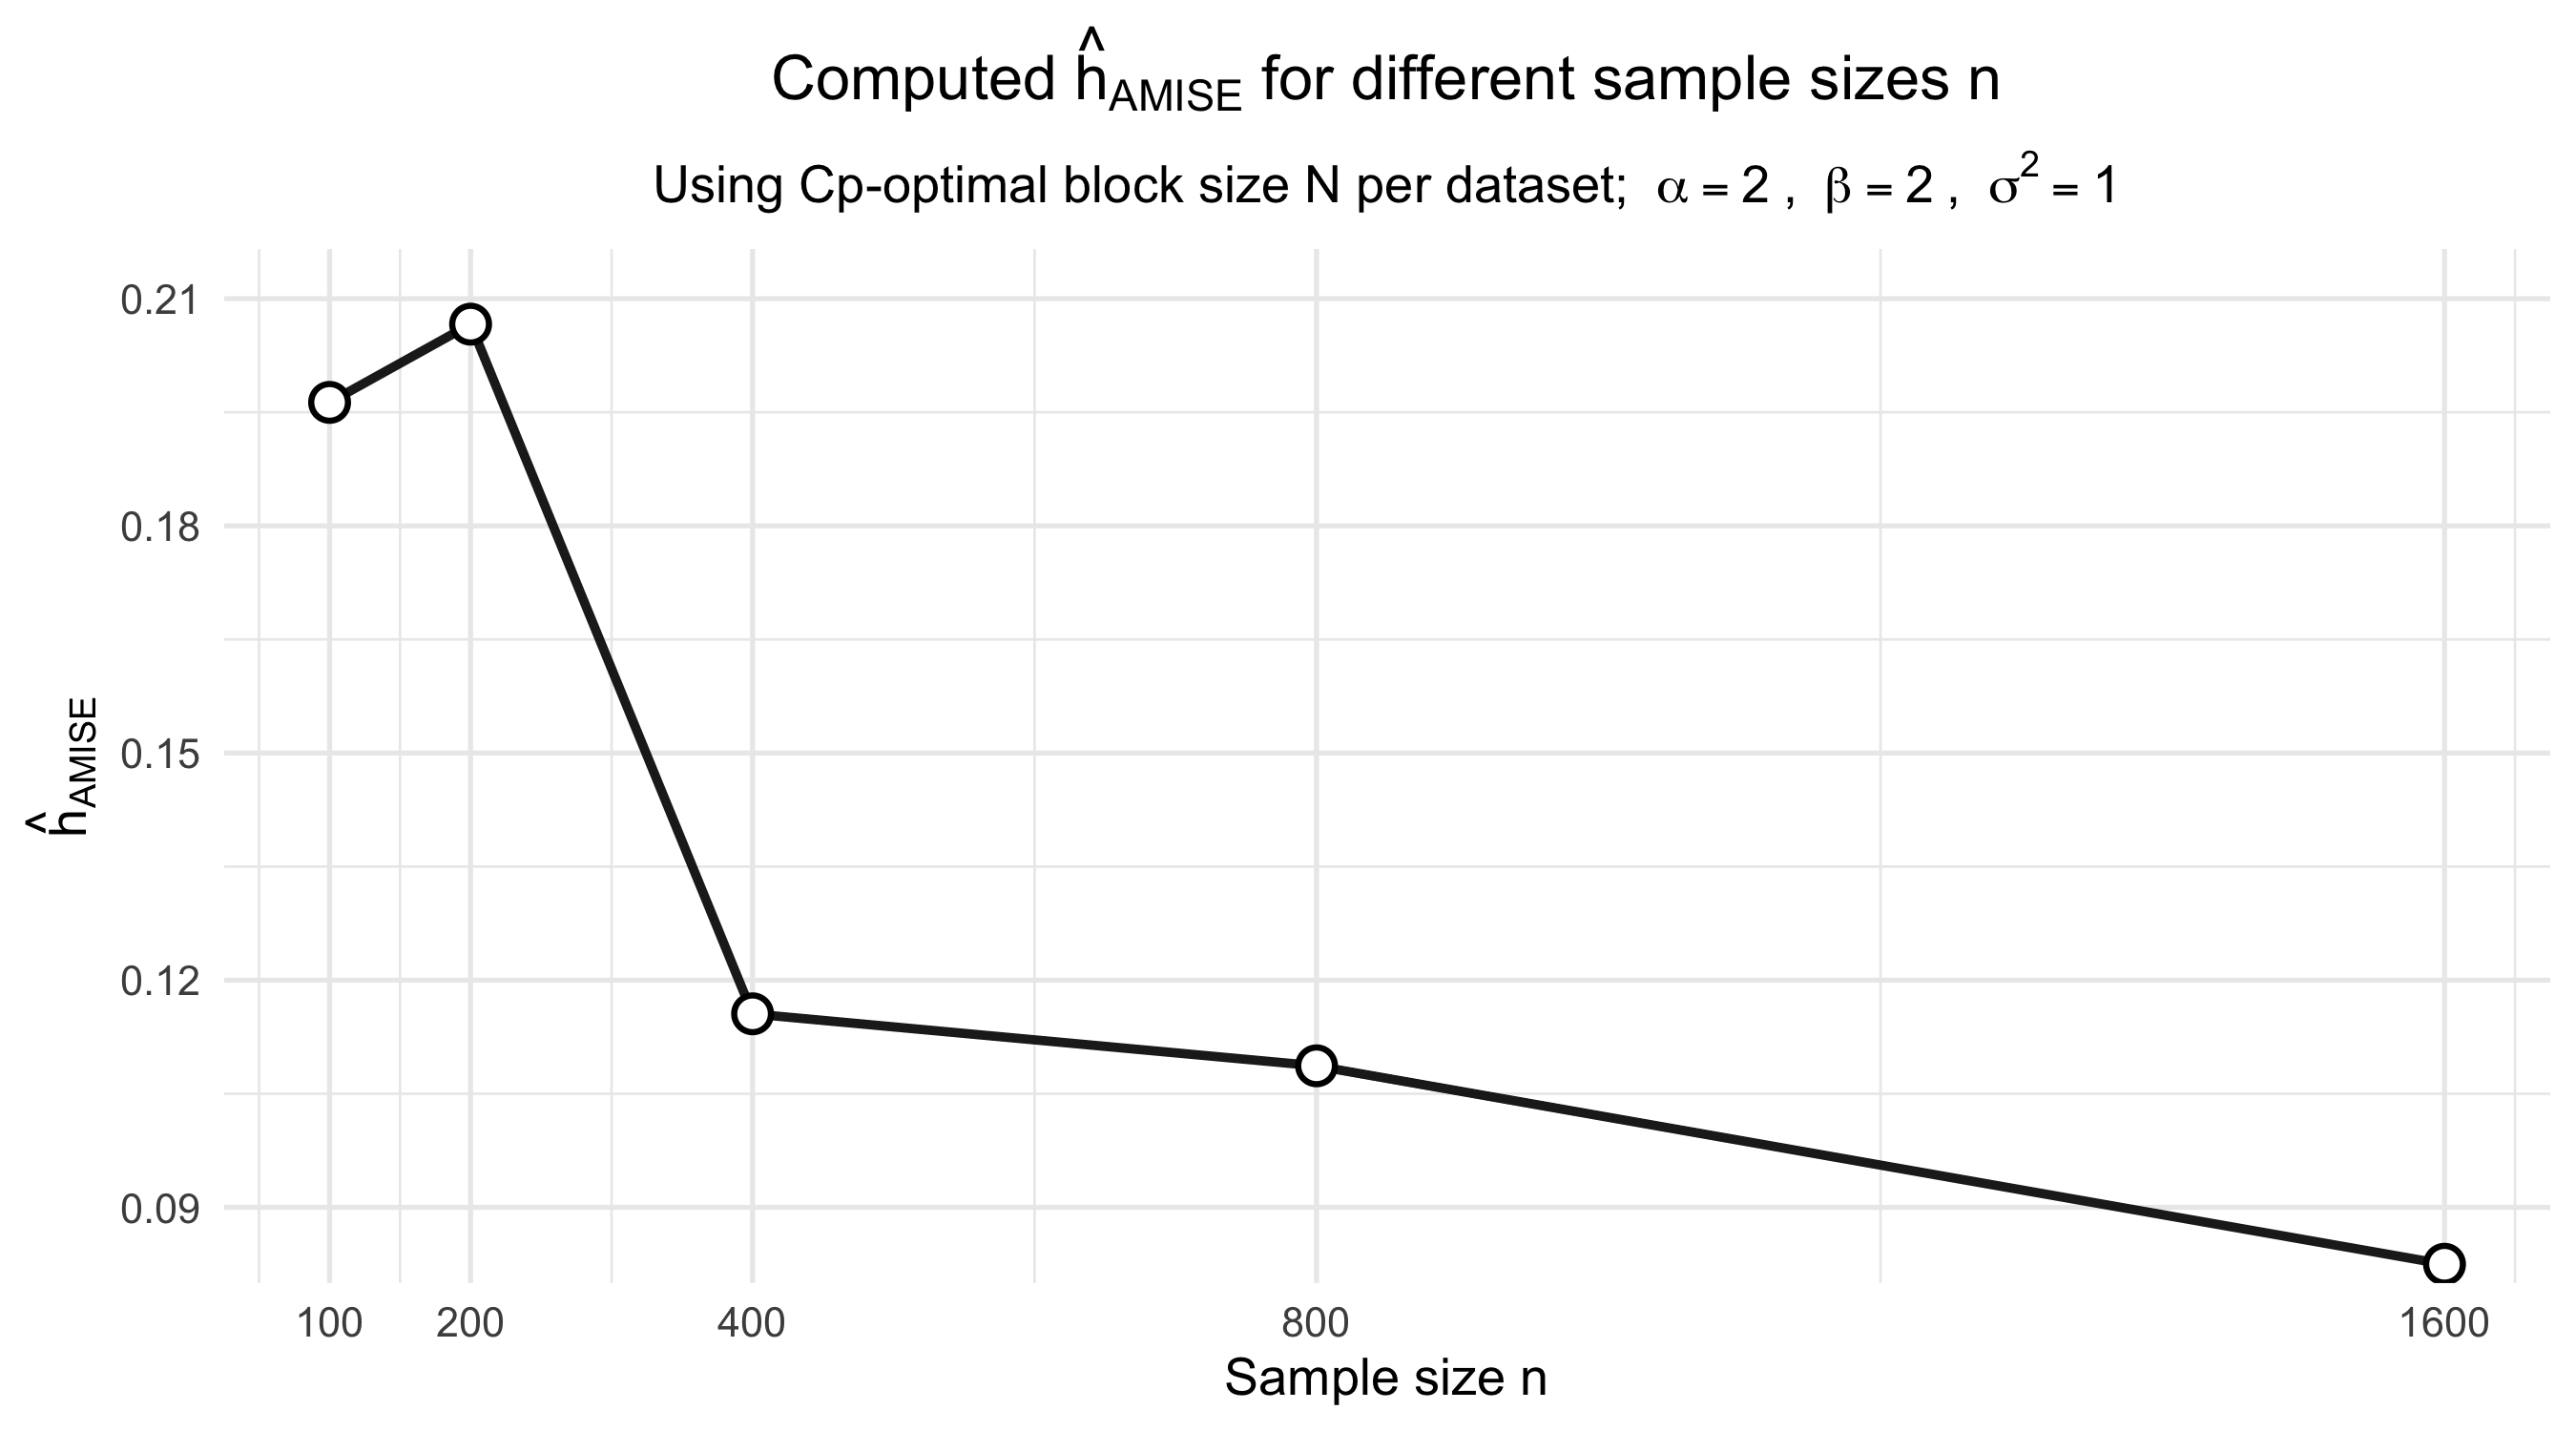
\includegraphics[keepaspectratio]{Single_Realization.png}}

}

\caption{Estimated optimal bandwidth h versus different sample sizes
n=100, 200, 400, 800 and 1600. The estimated bandwidth seems to decrease
as the sample size increases, which is what we expected would happen.}

\end{figure}%

While it does look like the estimated bandwidth \(\hat{h}_{AMISE}\)
shrinks as the sample size \(n\) grows, it is difficult to see where our
theoretical \(2^{-1/5}\) is. A more helpful way of looking at this would
be by taking the log-log scale:

\begin{figure}[H]

{\centering \pandocbounded{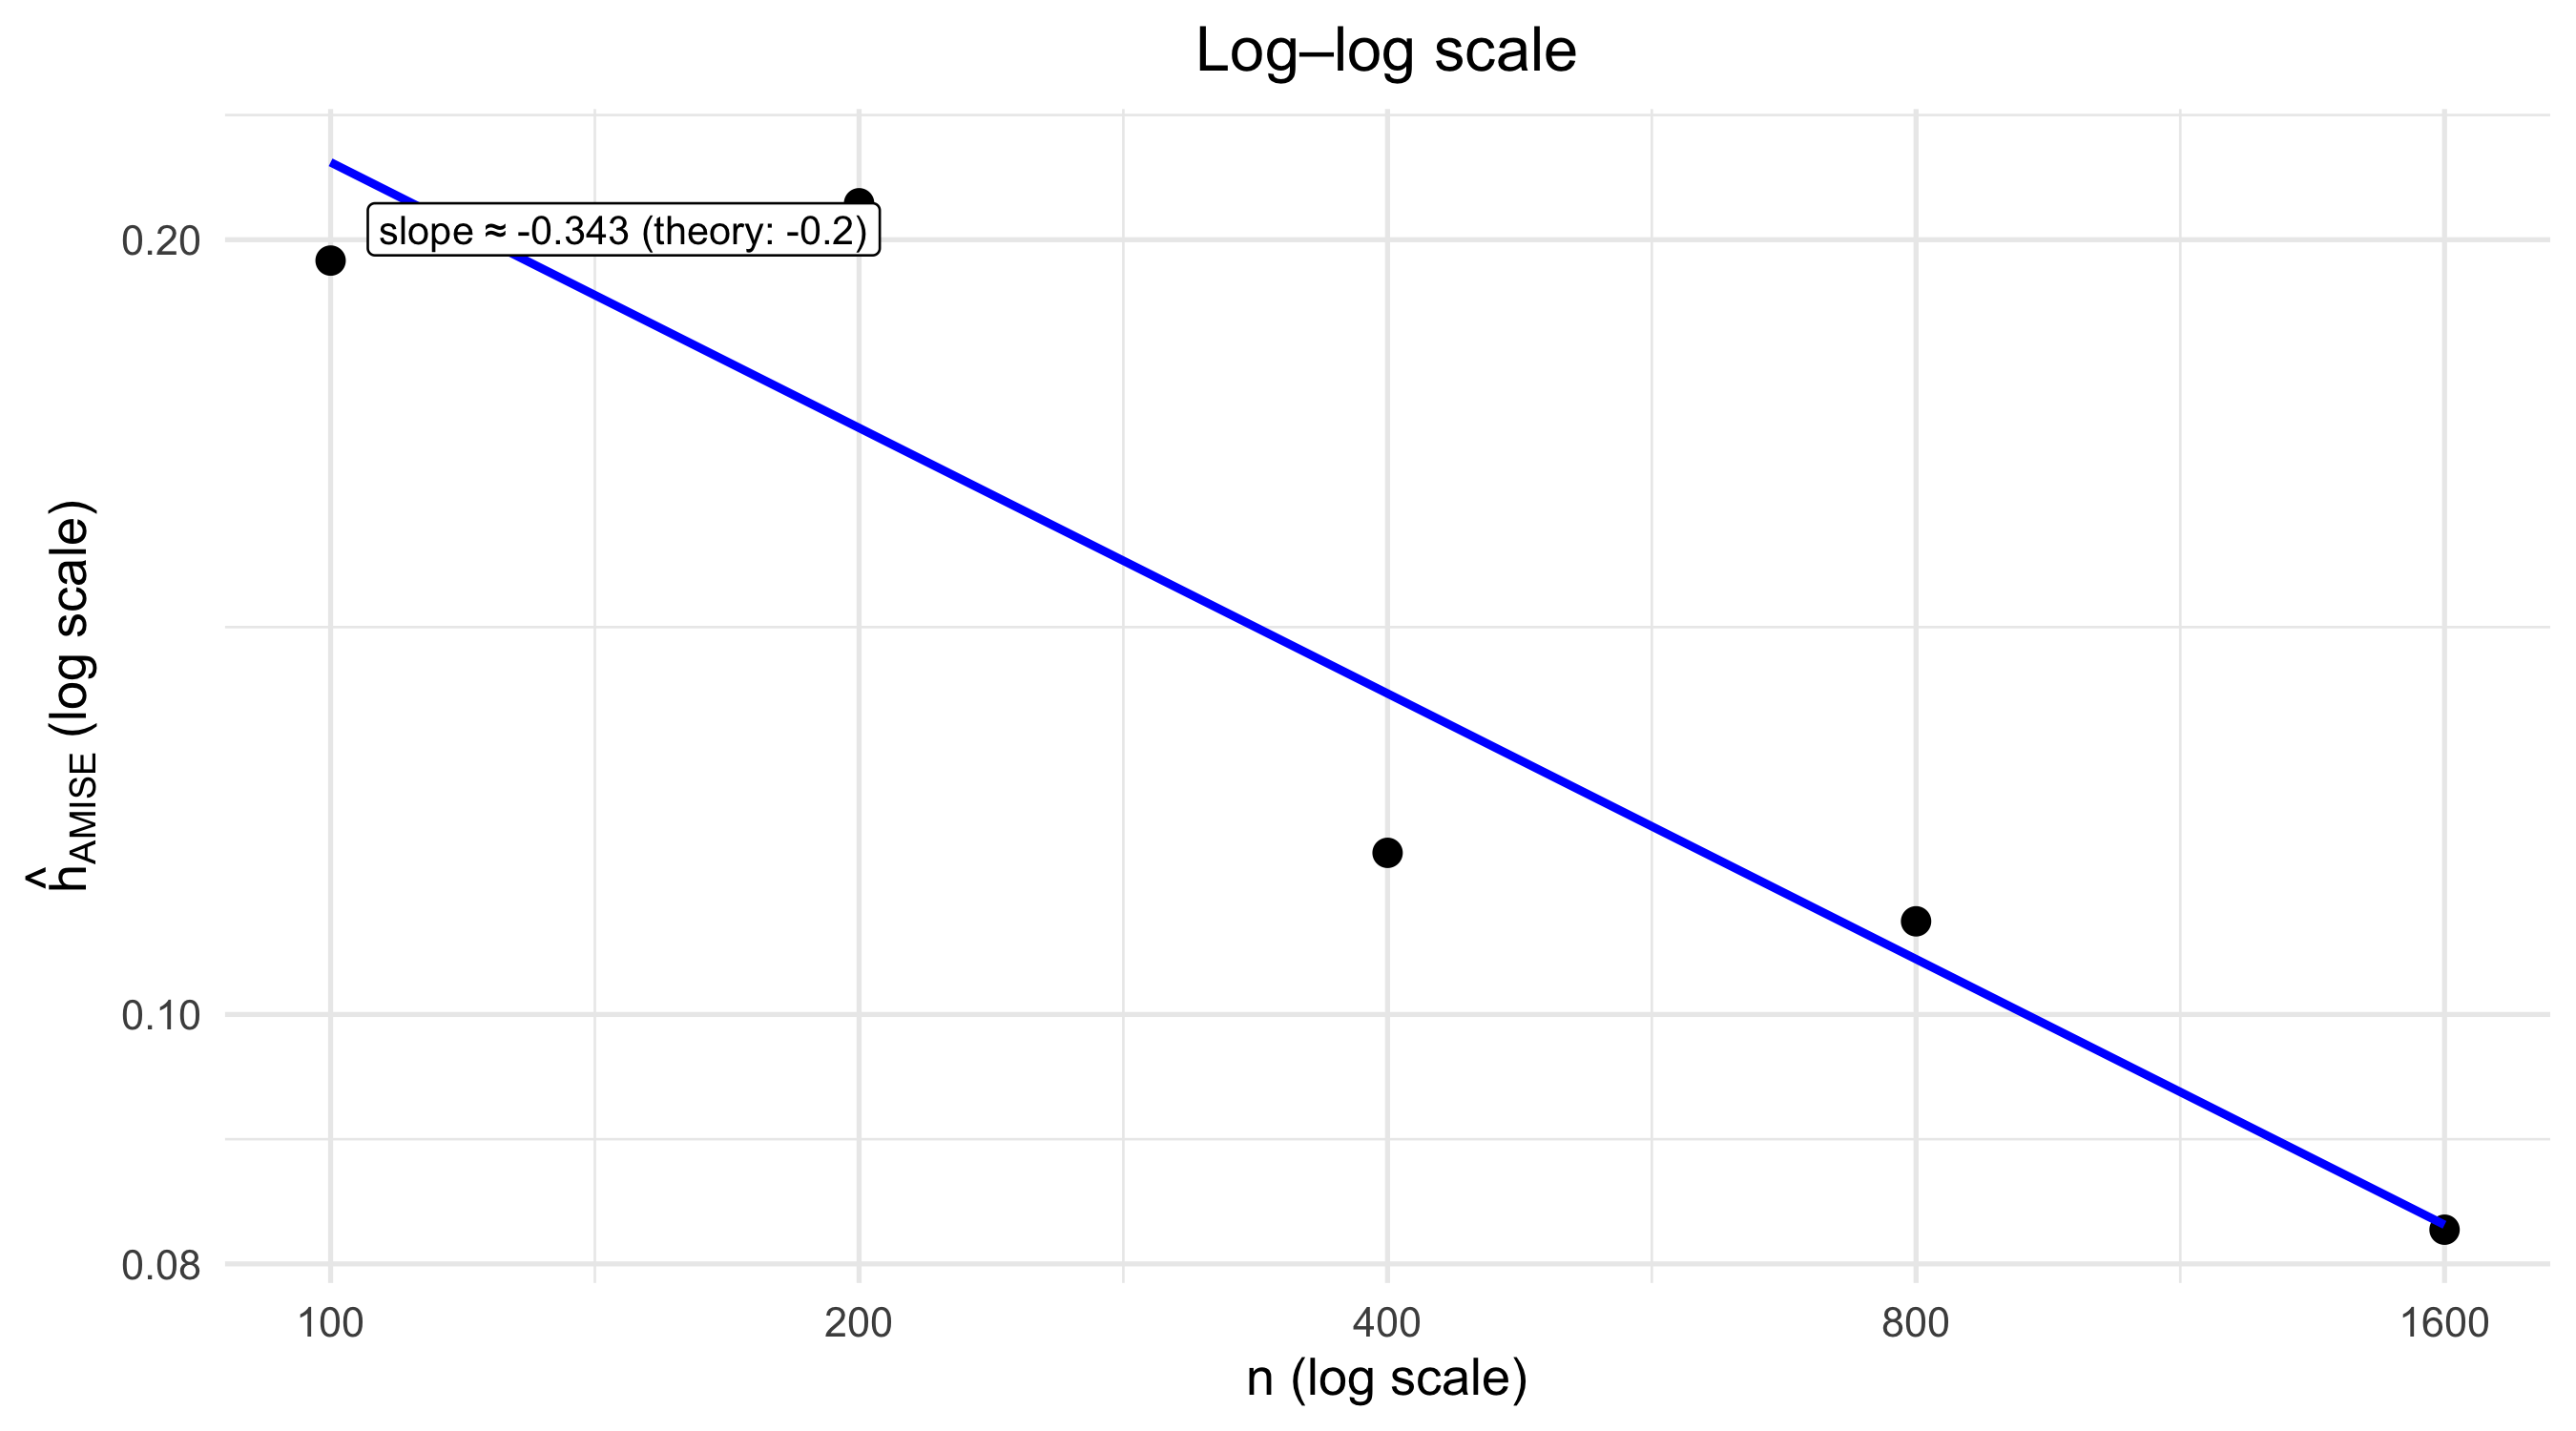
\includegraphics[keepaspectratio]{log_scale_plot.png}}

}

\caption{Log--log scaling of the plug-in bandwidth estimate
\(\hat{h}_{\mathrm{AMISE}}\) versus sample size \(n\). Each point is an
estimate computed for a given \(n\) (using the \(C_p\)-optimal block
size \(N\) for that dataset). The straight line is an OLS fit in
log--log space; its slope (shown on the plot) is close to the
theoretical \(-0.2\), confirming the expected scaling
\(\hat{h}_{\mathrm{AMISE}} \propto n^{-1/5}\). Axes are \(\log(n)\) and
\(\log(\hat{h}_{\mathrm{AMISE}})\).}

\end{figure}%

We repeat the simulation \(R = 400\) times for each sample size \(n\).
In each replicate, we resample \((X,Y)\), select the Cp-optimal block
size \(N\), and compute \(\hat{h}_{\text{AMISE}}\).

\begin{figure}[H]

{\centering \pandocbounded{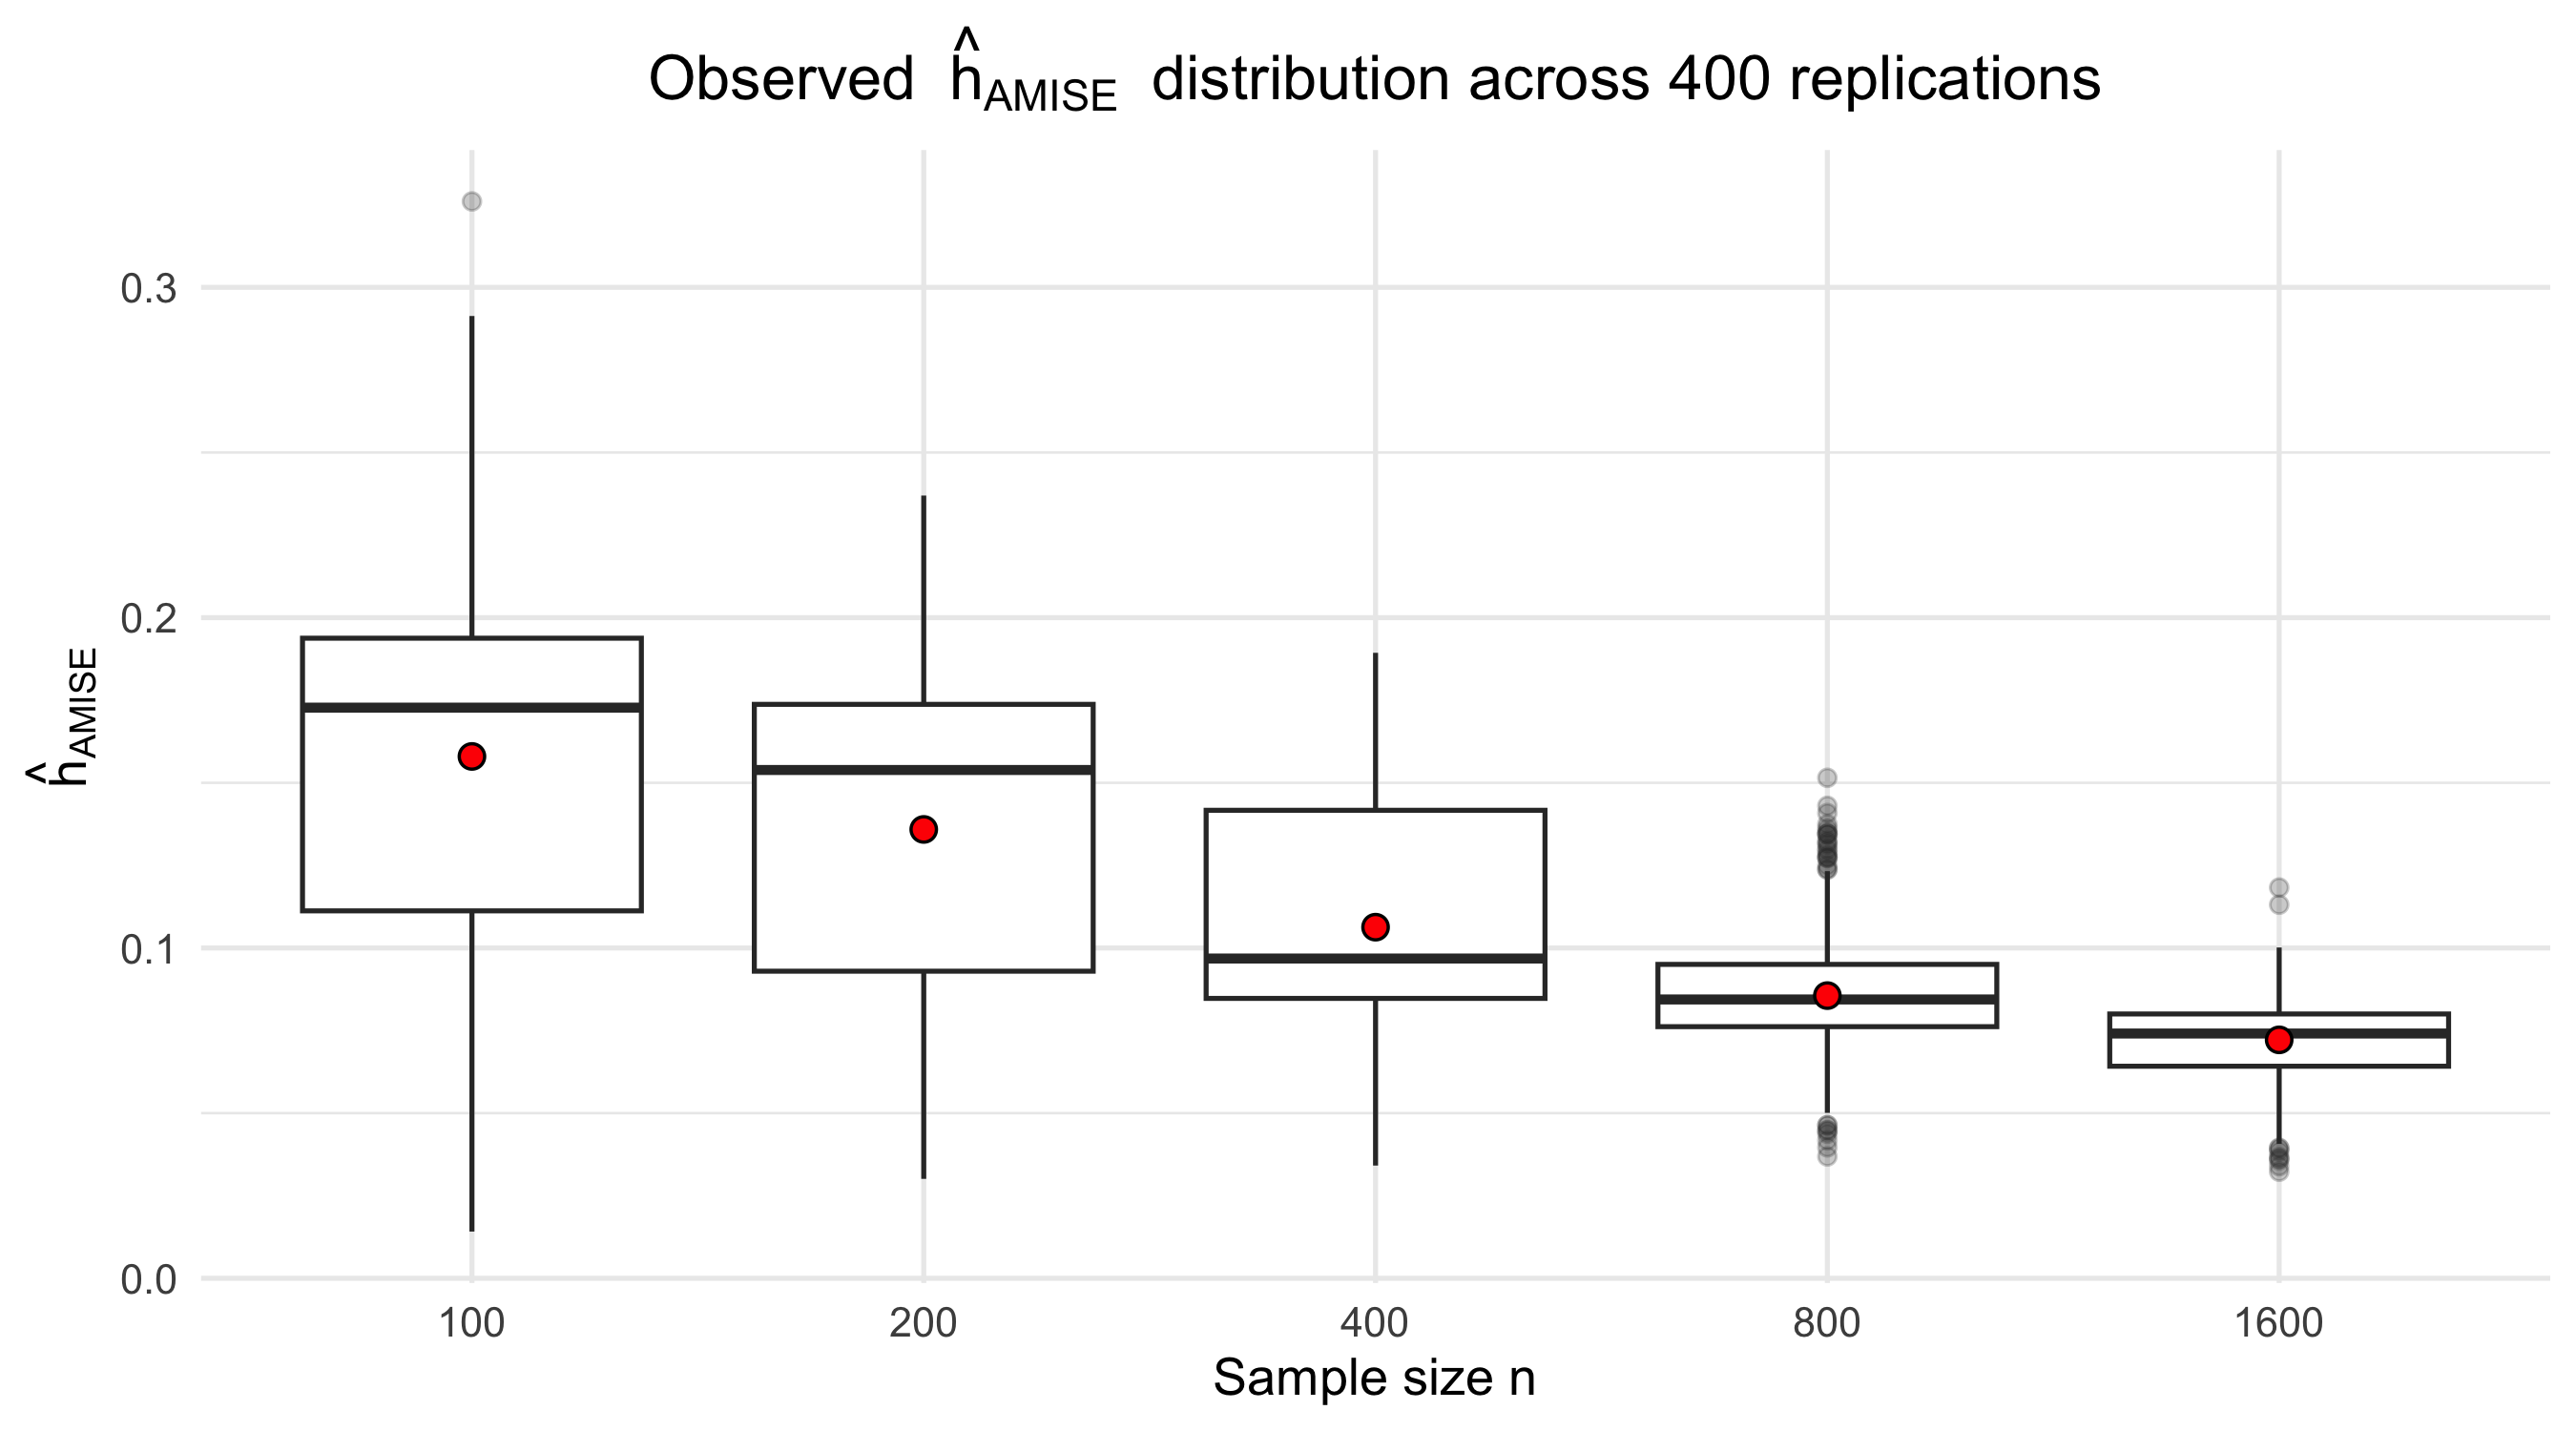
\includegraphics[keepaspectratio]{400_Replications.png}}

}

\caption{Boxplots of the plug-in bandwidth estimates
\(\hat{h}_{\text{AMISE}}\) across \(R=400\) replications for each sample
size \(n \in \{200,400,800,1600\}\). In each replicate we resample
\((X,Y)\), choose the Cp-optimal block size \(N\), and compute
\(\hat{h}_{AMISE}\). The overlaid dot indicates the mean across
replications.}

\end{figure}%

The boxplots above summarize the distribution across replications, which
gives a clear view of variability. The red dots indicate the means
across replications. Proceding as before, we get the following plot on a
log-log scale:

\begin{figure}[H]

{\centering \pandocbounded{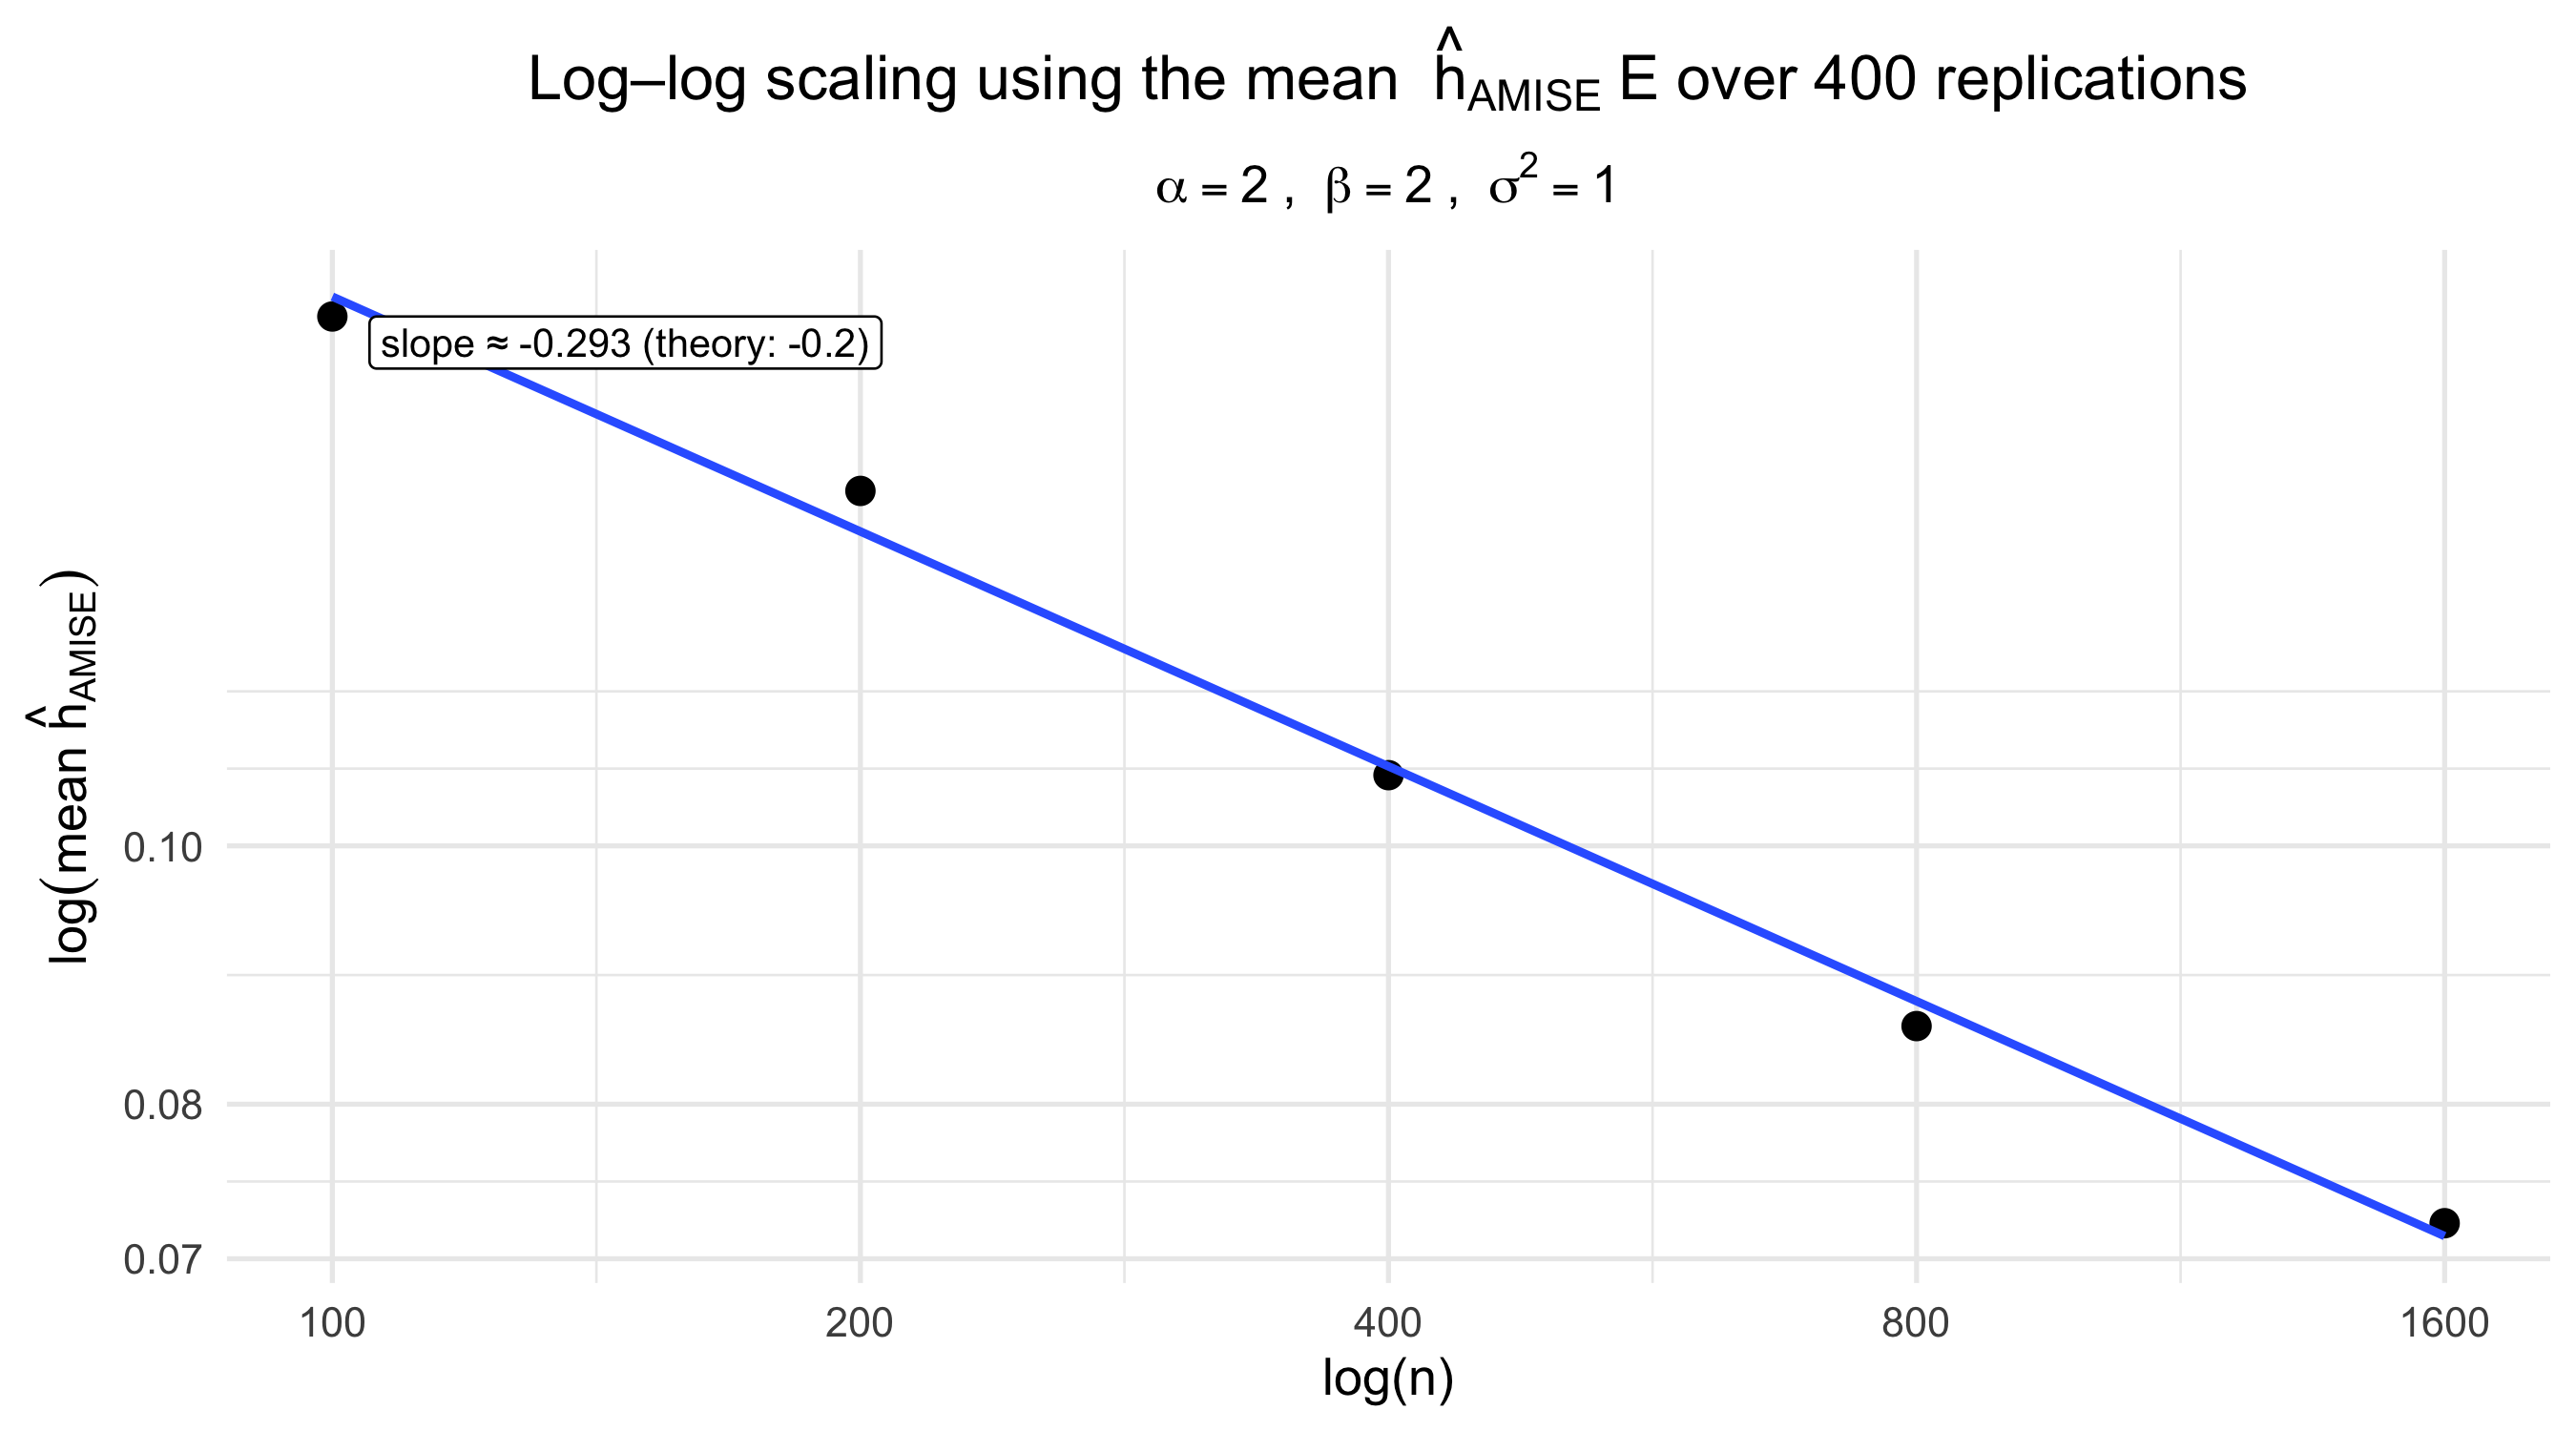
\includegraphics[keepaspectratio]{400_Replications_log_log.png}}

}

\caption{This plot shows \(\log(\overline{\hat{h}}_{\mathrm{AMISE}})\)
versus \(\log(n)\), where \(\overline{\hat{h}}_{\mathrm{AMISE}}\) is the
mean over \(R=400\) replications at each sample size
\(n \in {200,400,800,1600}\). In each replicate we resample \((X,Y)\),
choose the \(C_p\)-optimal block size \(N\), and compute
\(\hat{h}_{\mathrm{AMISE}}\). The straight line is an OLS fit in
log--log space; its slope is close to the theoretical \(-0.2\),
confirming \(\hat{h}_{\mathrm{AMISE}} \propto n^{-1/5}\).}

\end{figure}%

This strengthens our previous assumption, namely, that
\(\hat{h}_{\mathrm{AMISE}} \propto n^{-1/5}\). Let us now quickly look
at how the optimal value of \(N\) evolves, when increasing \(n\):

\begin{figure}[H]

{\centering \pandocbounded{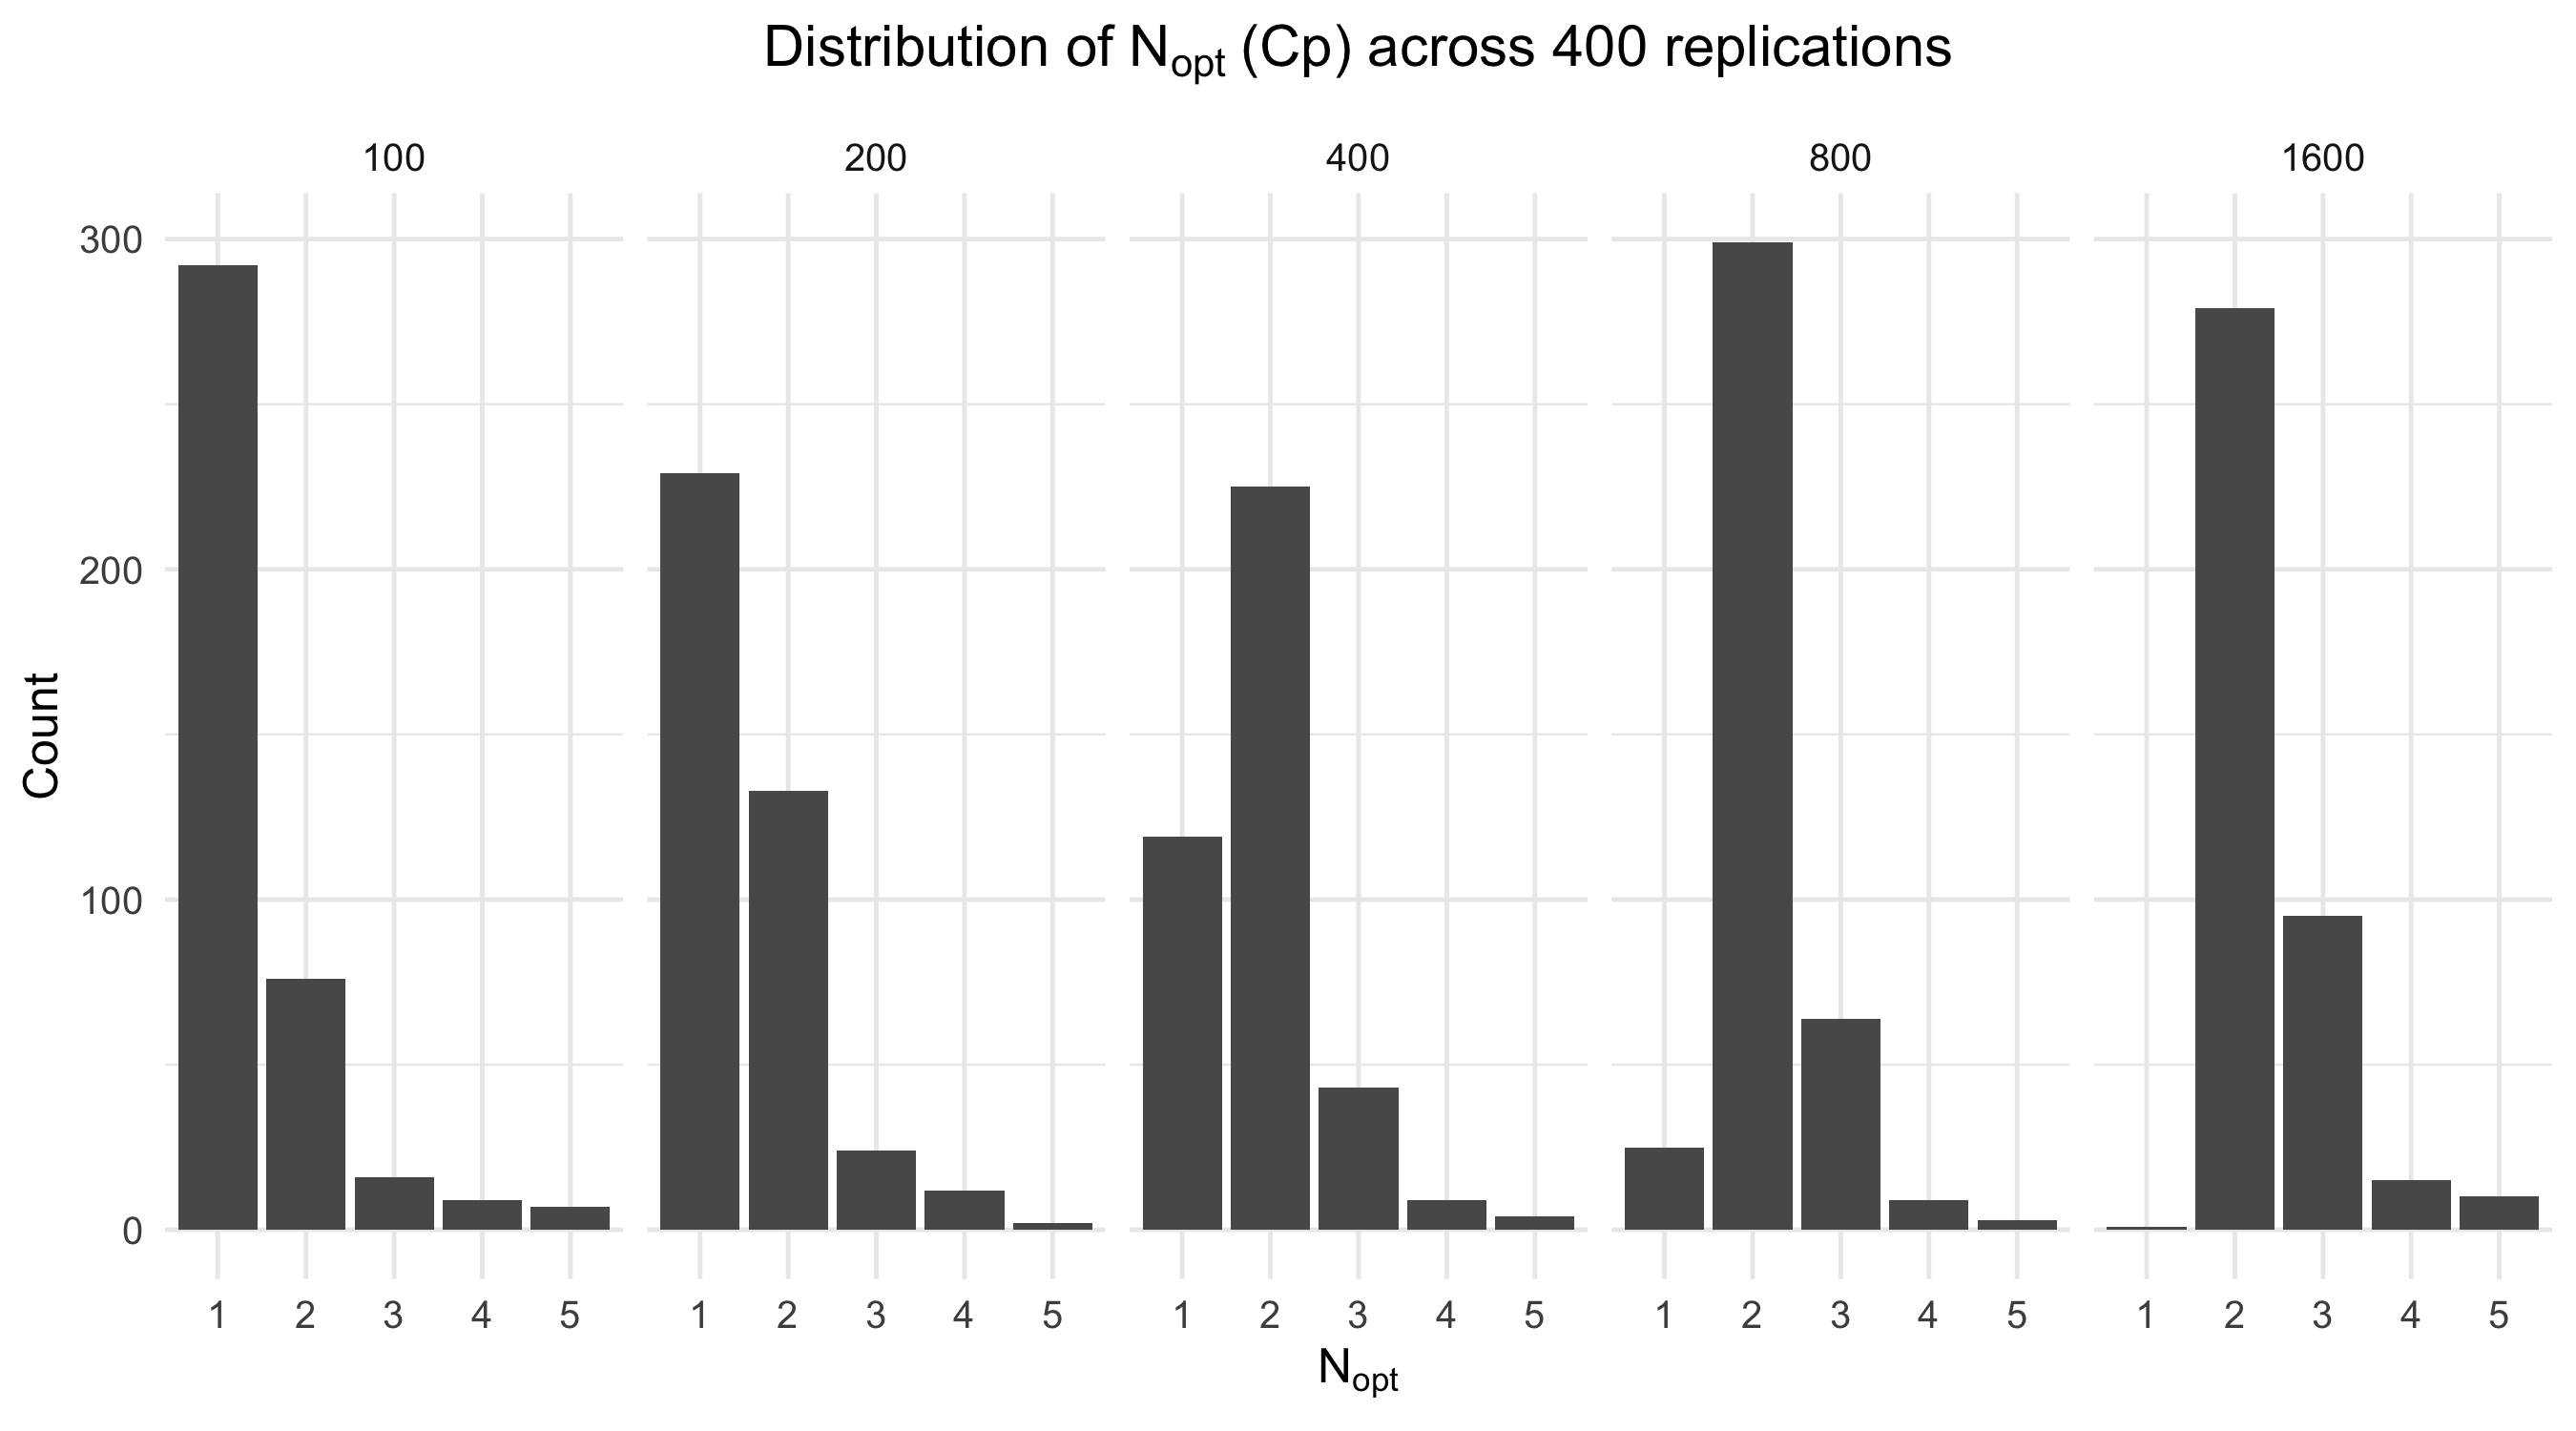
\includegraphics[keepaspectratio]{400_rep_N_vs_n.png}}

}

\caption{Estimated \(\hat{h}_{\mathrm{AMISE}}\) vs.~block size \(N\) by
sample size \(n\). Red points show the estimates computed from blockwise
degree-4 fits for each block size \(N\); the dashed vertical line in
each panel marks the value of \(N\) that minimizes Mallows' \(C_p\).''}

\end{figure}%

From this, it seems like \(N\) should depend on the sample size \(n\).
Indeed, each block fit uses \(5\) parameters, so we require \(n-5N>0\)
and a sufficient number of observations \emph{per block} (practically
\(\gtrsim 10\)--\(15\) in the sparsest block) for stable estimation. As
\(n\) increases we can afford a larger \(N\) without starving blocks;
empirically the \(C_p\)--optimal \(\hat N_{\text{opt}}\) increases
slowly with \(n\). We now want to look into the impact the chosen block
size \(N\), used in the estimation of \(\theta_{22}\) and \(\sigma^2\),
has on the estimate \(\hat{h}_{AMISE}\). We will this time let the
sample size take the values \(200, 800, 3200\) and \(12800\). Moreover,
for each \(n\), we let \(N \in \{1, \ldots, N_{\max} \}\).

\begin{figure}[H]

{\centering \pandocbounded{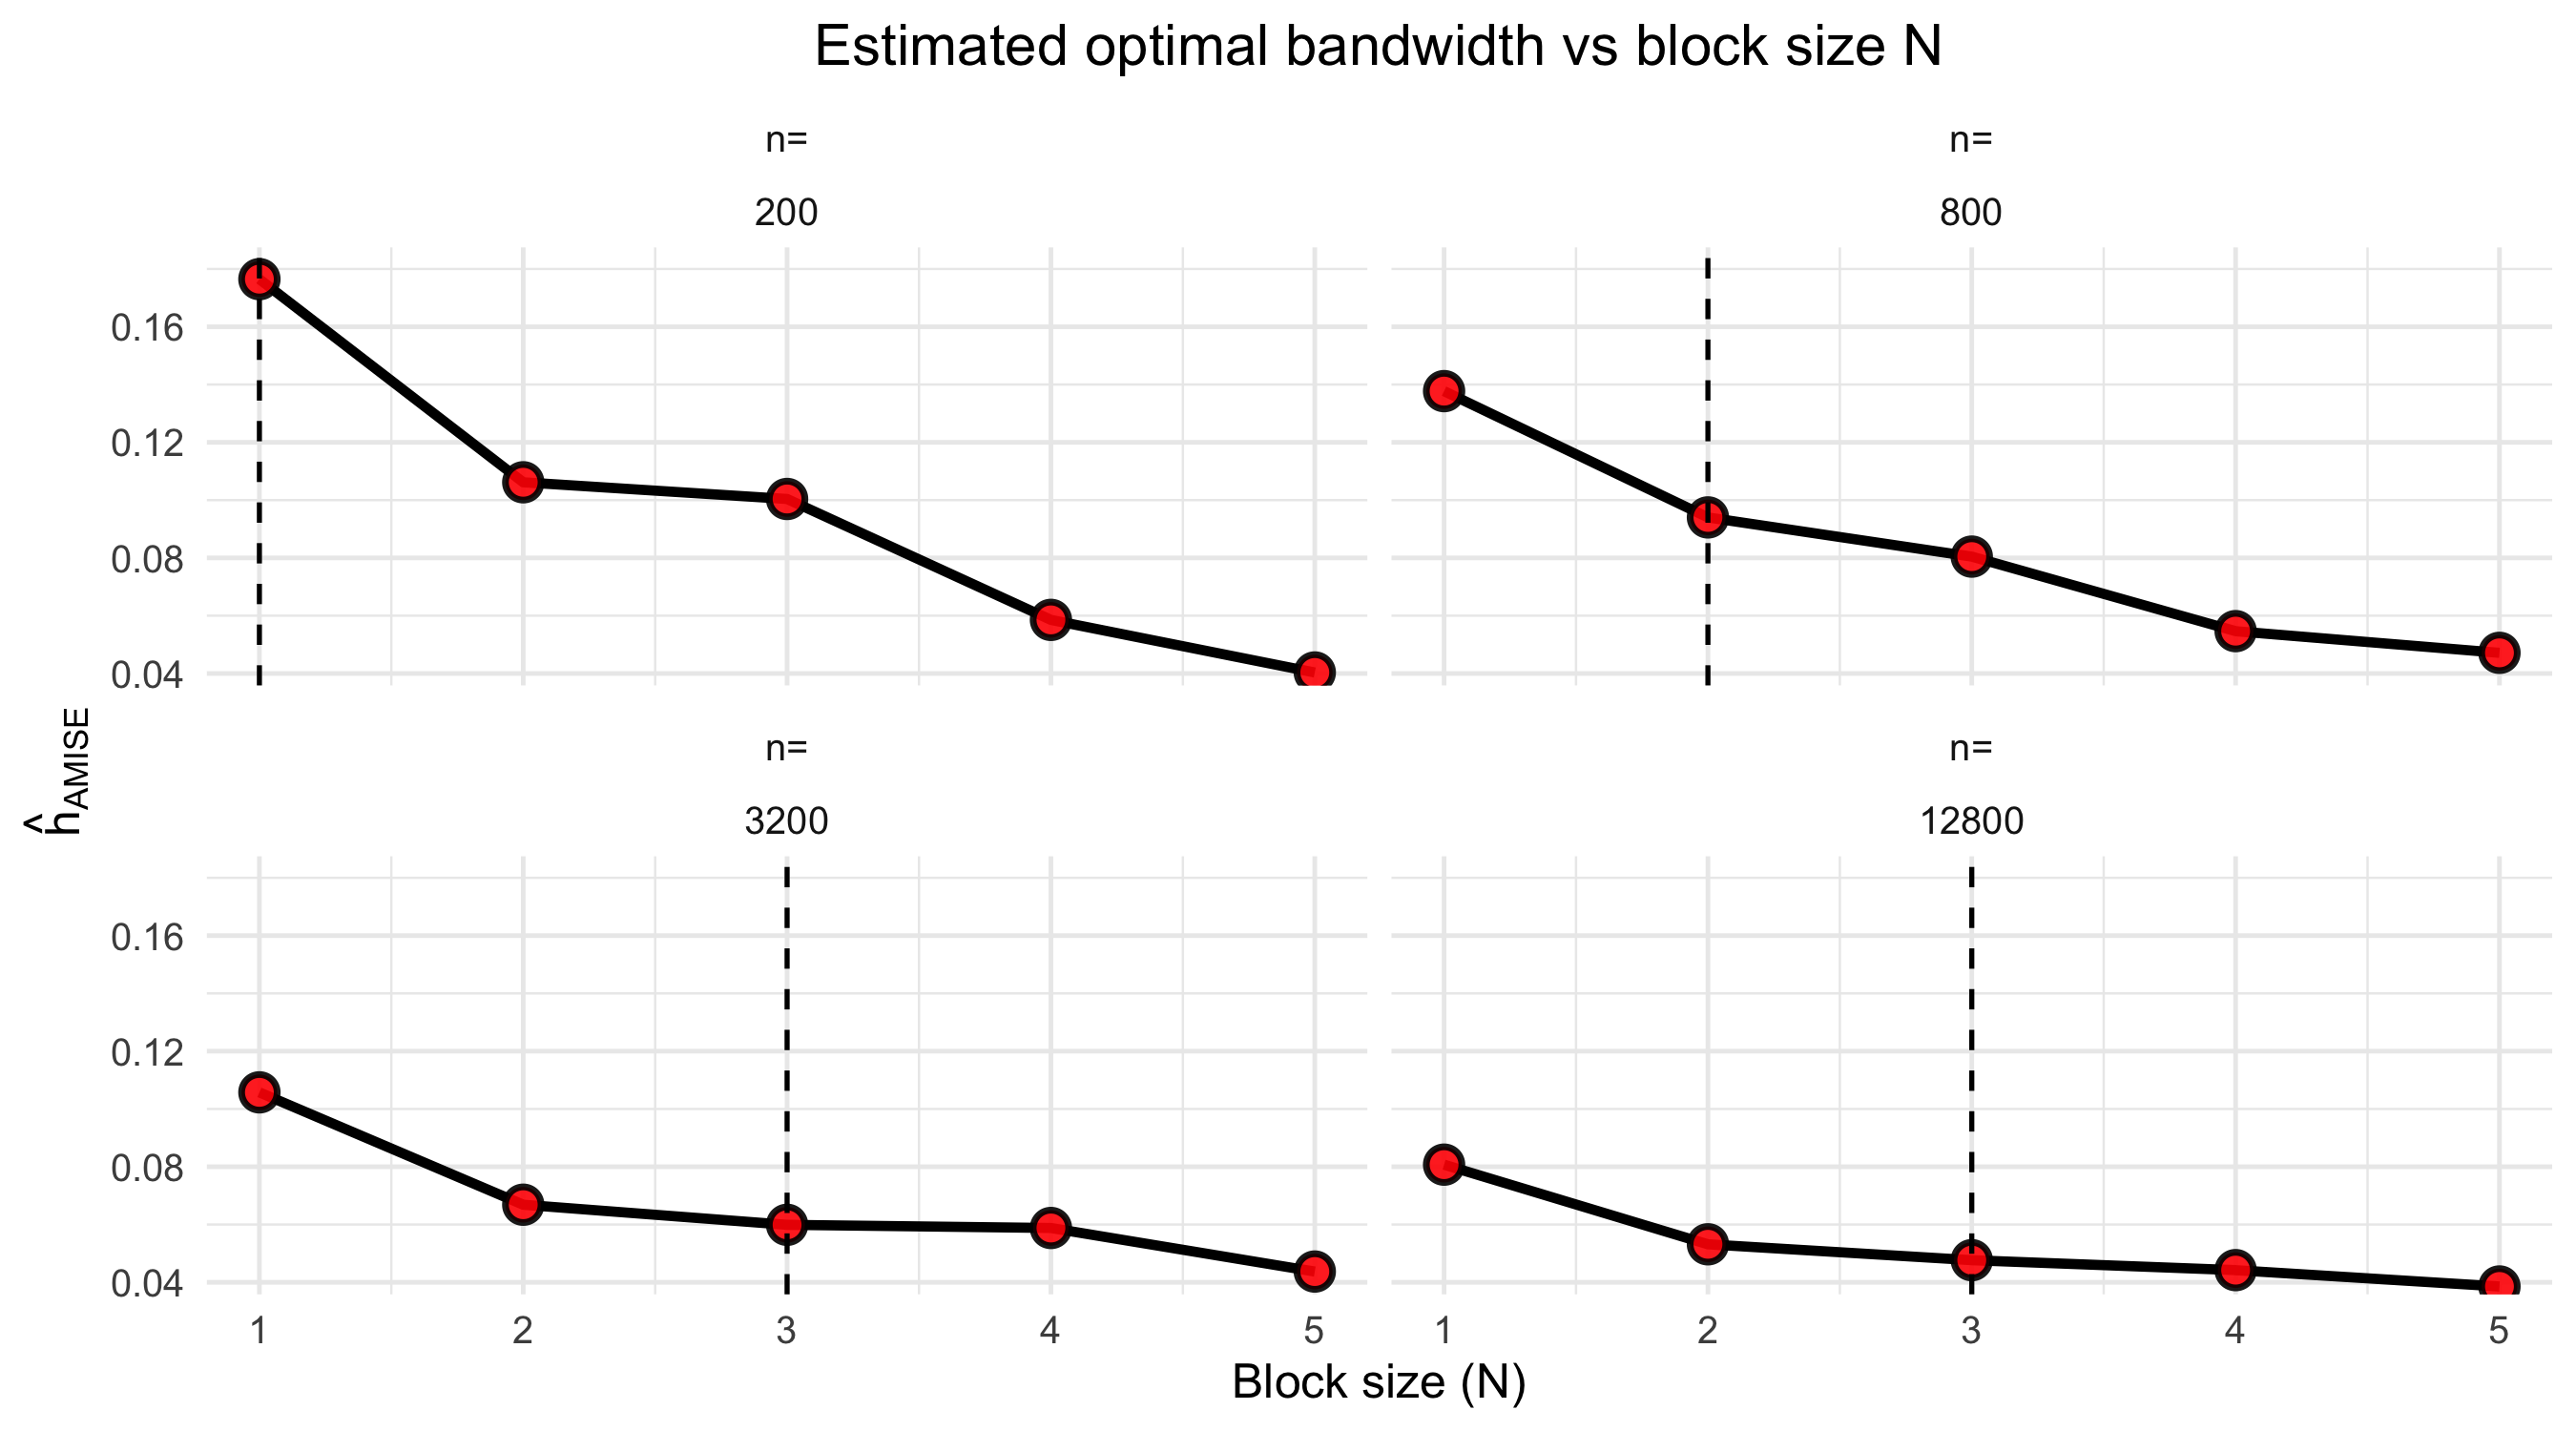
\includegraphics[keepaspectratio]{bandwidth_vs_N.png}}

}

\caption{Estimated \(\hat{h}_{\mathrm{AMISE}}\) vs.~block size \(N\) by
sample size \(n\). The red points show the estimates computed from
blockwise degree-4 fits for each block size \(N\) ; the dashed vertical
line in each panel marks the value of \(N\) that minimizes mallow's
\(C_p\).}

\end{figure}%

For very small \(N\), the blockwise degree--4 polynomials underfits the
regression function \(m(\cdot)\), which downplays our estimate
\(\hat{\theta}_{22}\) and inflates the variance estimate
\(\hat{\sigma}}^2\). Since \$ \hat h\_\{\mathrm{AMISE}\}
\propto \Big(\dfrac{\hat{\sigma}^2}{\hat{\theta}_{22}}\Big)\^{}\{1/5\},\$
the ratio is large and \(\hat h\) is too big. Increasing \(N\) improves
curvature capture, raising \(\hat{\theta}_{22}\) and reducing
\(\hat{\sigma}^2\), so \(\hat h\) decreases. When increasing \(N\), some
blocks become saprse and the residual degrees of freedoms \(n-5N\)
shrinks, making both \(\hat{\theta}_{22}\) and \(\hat{\sigma}^2\) more
noisy.

Lastly, we want to explore the effects different values of the
parameters \(\alpha\) and \(\beta\) have on our estimate
\(\hat{h}_{AMISE}\). We fix \(n=1600\) and take \(N_p\), the value of
\(N\) minimizing Mallow's \(C_p\), as the block size.

\begin{figure}[H]

{\centering \pandocbounded{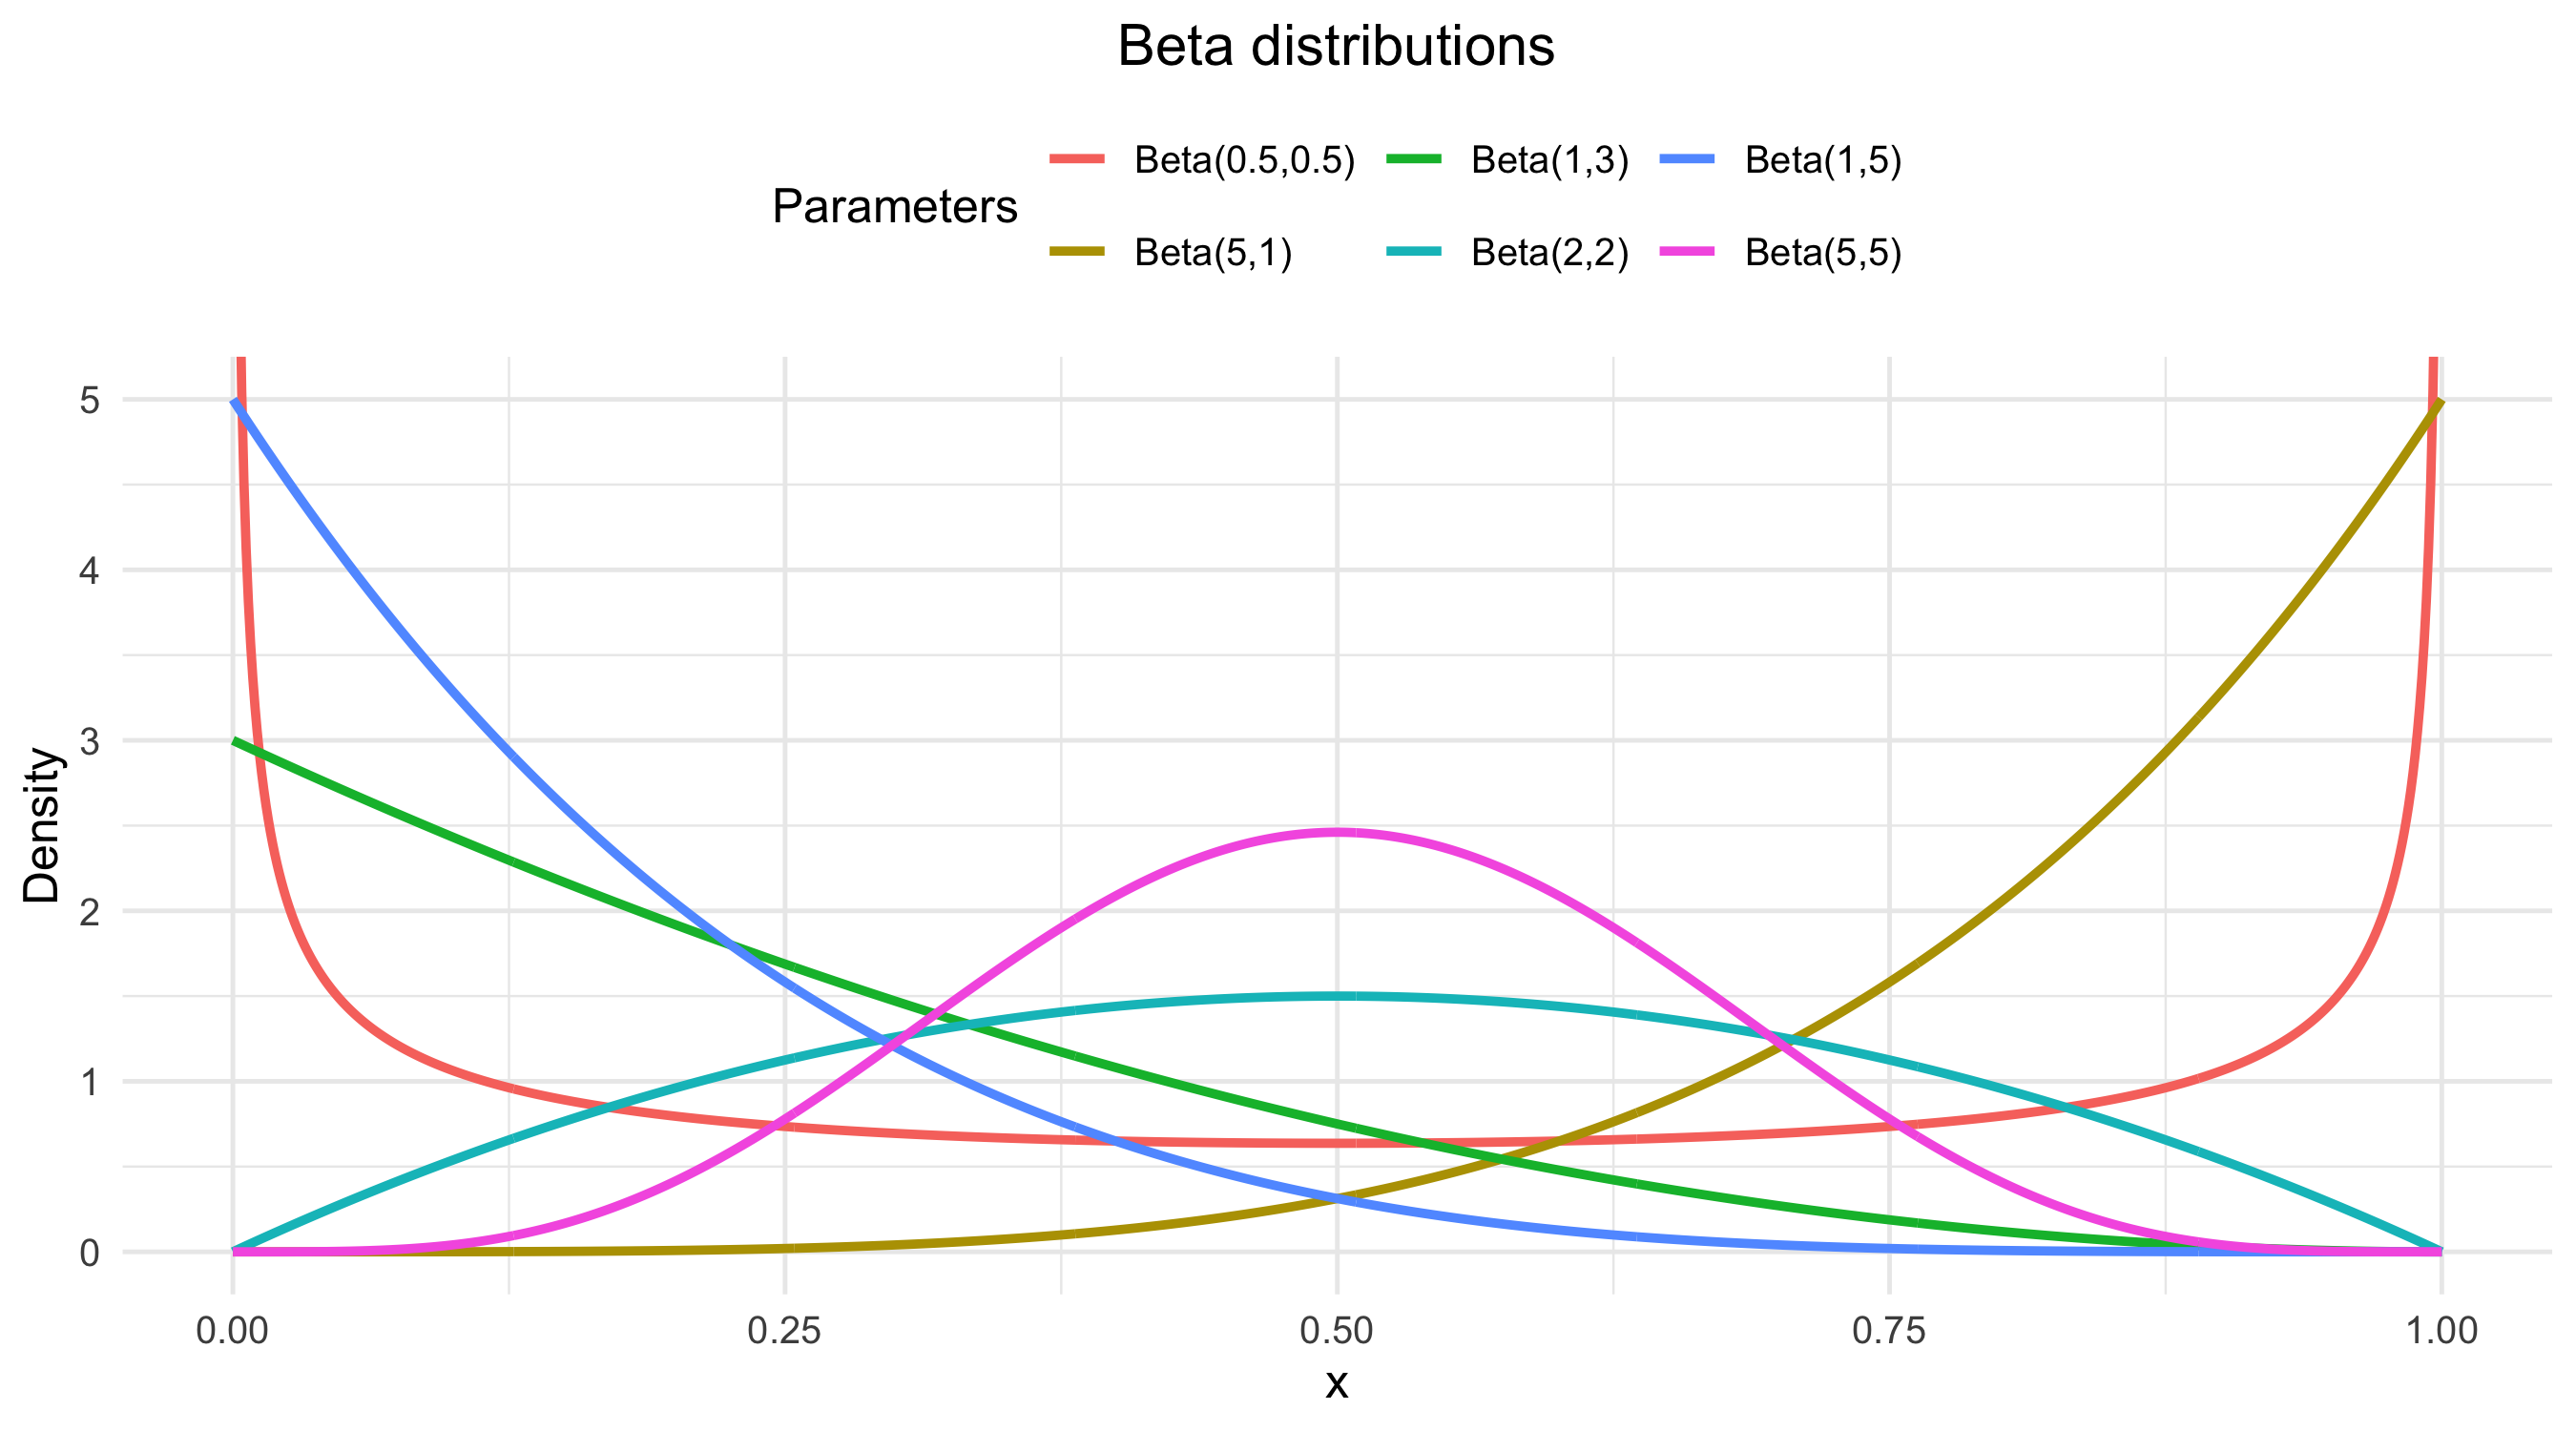
\includegraphics[keepaspectratio]{pdf_beta_shapes.png}}

}

\caption{Probability density function of the Beta\((\alpha, \beta)\)
distribution for different pairs \((\alpha, \beta)\).}

\end{figure}%

The above plot shows how the shape of the Beta density changes with
\((\alpha,\beta)\), when \((\alpha,\beta) = (0.5, 0.5)\), we get a
U--shaped density and when \(\alpha\neq\beta\), we get strong skews, and
parts of \([0,1]\) become sparsely populated as a consequence. This has
a significant impoact on our estimator of the optimal bandwidth as with
equal--width blocks, those regions translate into sparse blocks, so the
degree--4 fits of \(\hat m\), and \(\hat m''\), performed in each block
are noisier. As a result, the plug--in estimators \(\hat\theta_{22}\)
and \(\hat\sigma^2\) fluctuate more and the resulting
\(\hat{h}_{\mathrm{AMISE}}\) varies more across replications. By
contrast, for more evenly spread designs (e.g., \(\mathrm{Beta}(2,2)\)
or \(\mathrm{Beta}(5,5)\)), blocks are better populated, the fits are
more stable, and the distribution of \(\hat{h}_{\mathrm{AMISE}}\) over
the 400 replications is noticeably tighter as we can see on the
following plot:hat

\begin{figure}[H]

{\centering \pandocbounded{\includegraphics[keepaspectratio]{boxplots_beta_shapes.png}}

}

\caption{The plot illustrates the distribution of the estimated
\(h_{AMISE}\) for different beta shapes (pairs (\(\alpha, \beta\))). As
expected, the estimated values of \(h_{AMISE}\) fall in a tighter
intervall when the corresponding density functions are more evenly
spread across \([0, 1]\).}

\end{figure}%




\end{document}
